% Preamble
% ---
\documentclass{article}

% Packages
% ---
\usepackage{amsmath} % Advanced math typesetting
\usepackage[utf8]{inputenc} % Unicode support (Umlauts etc.)
\usepackage[T1]{fontenc}
\usepackage{biolinum}
\usepackage[ngerman]{babel} % Change hyphenation rules
\usepackage[autostyle]{csquotes}
\usepackage{hyperref} % Add a link to your document
\usepackage{graphicx} % Add pictures to your document
\usepackage{listings} % Source code formatting and highlighting
\usepackage{fancyhdr}
\usepackage{biblatex}
\usepackage{pgfplots}
\usepackage{txfonts}
\usepackage{caption}

\author{Clemens Dautermann}
\title{\Huge Grundbegriffe des maschinellen Lernens} 
\date{\today{}}
\pagestyle{fancy}
\captionsetup{justification=raggedright,singlelinecheck=false}



\begin{document}
\biolinum
\pagenumbering{gobble}
\begin{titlepage}
	\maketitle
\end{titlepage}
\pagenumbering{arabic}
\tableofcontents{}
\newpage

\section{Was ist maschinelles Lernen?}
Die wohl bekannteste und am häufigsten zitierte Definiton des maschinellen Lernens stammt von Arthur Samuel aus dem Jahr 1959. Er war Pionier auf diesem Gebiet und rief den Begriff \glqq machine learning'' ins Leben. So sagte er:
\begin{quote}
	[Machine learning is the] field of study that gives computers the ability to learn without being explicitly programmed\cite{1}.
	\begin{flushright}
		---Arthur Samuel, 1959
	\end{flushright}
\end{quote}
Beim maschinellen lernen werden Computer also nicht mit einem bestimmten Algorythmus programmiert um eine Aufgabe zu lösen, sondern lernen eigenständig diese Aufgabe zu bewältigen. Dies geschieht zumeist, indem das Programm aus einer großen, bereits \glqq gelabelten'', Datenmenge mit Hilfe bestimmter Methoden, die im Folgenden weiter erläutert werden sollen, lernt, gewisse Muster abzuleiten um eine ähnliche Datenmenge selber \glqq labeln'' zu können.  Als Label bezeichent man in diesem Fall die gewünschte Ausgabe des Programmes. Dies kann beispielsweise eine Klassifikation sein. Soll das Programm etwa handgeschriebene Ziffern erkennen können, so bezeichnet man das (bearbeitete) Bild der Ziffer als \glqq Input Verctor'' und die Information welche Ziffer der Copmputer hätte erkennen sollen, als \glqq Label ''. Soll jedoch maschinell erlernt werden, ein simuliertes Auto zu fahren, so bestünde der Input Vector aus Sensorinformationen und das Label würde aussagen, in welche Richtung das Lenkrad hätte gedreht werden sollen, wie viel Gas das Programm hätte geben sollen oder andere Steuerungsinformationen. Der Input Vector ist also immer die Eingabe, die der Computer erhält um daraus zu lernen und das Label ist die richtige Antwort, die vom Programm erwartet wurde. Für maschinelles Lernen wird also vor allem eins benötigt: Ein enormer Datensatz, der bereits gelabelt wurde, damit das Programm daraus lernen kann.\newline
Natürlich werden für maschinelles Lernen trotzdem Algorythmen benötigt. Diese Algorythmen sind jedoch keine problemspezifischen Algorythmen, sondern Algorythmen für maschinelles Lernen. Eine der populärsten Methoden des maschinellen Lernens ist das sogenannte \glqq Neuronale Netz''. 
\subsection{Klassifizierungsprobleme}
\subsection{Regressionsprobleme}
\subsection{Gefahren von maschinellem Lernen}
\subsubsection{Eignung der Datensätze}
\subsubsection{Overfitting}
\subsubsection{Unbewusste Manipulation der Daten}
\section{Verschiedene Techniken maschinellen lernens}
\subsection{Überwachtes Lernen}
\subsection{Unüberwachtes Lernen}
\subsection{Bestärkendes Lernen}
\section{Neuronale Netze}
bei Neuronalen Netzen handelt es sich um eine programminterne Struktur, die für das maschinelle Lernen genutzt wird. Wie der Name bereits vermuten lässt, ist diese Methode ein Versuch das menschliche Lernen nachzuahmen.
\subsection{Maschinelles Lernen und menschliches Lernen}
Das menschliche Gehirn ist aus sogenannten \glqq Neuronen'' aufgebaut. Ein Neuron ist eine Nervenzelle, die elektrische oder chemische Impulse annimmt, und gegebenenfalls einen elektrischen oder chemischen Impuls weitergibt. Die Nervenzellen berühren sich nicht direkt sondern sind nur über die sogenannten Synnapsen verbunden, über die diese Signale übertragen werden, sodass sich ein hoch komplexes Netzwerk von milliarden von Neuronen ergibt.\footnote{
Diese Definition ist stark vereinfacht. Sie enthält ausschließlich die wesentlichen Komponenten um das menschliche Gehirn mit einem neuronalen Netz vergleichen zu können.}
\begin{figure}[h]
	\centering
	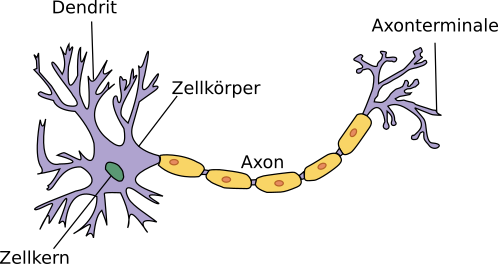
\includegraphics[]{../graphics/Neuron.png}
	\caption[Neuron \newline 
	Quelle: simple.wikipedia.org/wiki/File:Neuron.svg\newline
	Copyright: CC Attribution-Share Alike von Nutzer Dhp1080,\newline
 	bearbeitet]{Ein Neuron wie es im Gehirn vorliegt}
\end{figure}
Ein neuronales Netz ist ähnlich aufgebaut. Es besteht aus \glqq Neuronen'', die eine theoretisch beliebige Anzahl von Eingaben annehmen können und mit einer entsprechenden Ausgabe reagieren, sowie Verbindungen zwischen den Neuronen. Auch das Lernprinzip entspricht dem eines Menschen. Das Netz nimmt immer Zahlen zwischen 0 und 1 als Eingabe an und berechnet eine entsprechende Ausgabe. Es erhält anschließend die Information, wie die richtige Lösung gelautet hätte und lernt dann aus seinen Fehlern, indem es gewisse Werte, die in die Berechnung einfließen, anpasst. Analog lernt ein Mensch, indem er ausprobiert, gegebenenfalls scheitert, anschließend die richtige Antwort durch eine externe Quelle erhält und somit aus seinem Fehler lernt. Im Menschlichen Gehirn verknüpfen sich Dabei oft genutzte neuronale Verbindungen stärker und weniger benutzte Verbindungen bauen sich ab\cite{2}. Die Verstärkung und der Abbau entsprechen dem Ändern der Gewichtung einer Verbindung im neuronalen Netz. Die Gewichtung ist eine Eigenschaft der Verbindung, die eine zentrale Rolle in der Berechnung spielt und soll im folgenden weiter erläutert werden. Diese Ähnlichkeiten sind kein Zufall, sondern viel mehr Intention. Ein neuronales Netz ist nämlich der gezielte Versuch das menschliche Lernen nachzuahmen um maschinelles Lernen zu ermöglichen.
\subsection{Der Aufbau eines neuronalen Netzes}
Ein neuronales Netz besteht aus Neuronen und Verbindungen zwischen diesen. Es gibt einen sogenannten \glqq Input Layer'', der die Daten, den sogenannten \glqq Input Vector'', annimmt, eine beliebige Anzahl von sogenannten \glqq Hidden Layers'', in denen das eigentliche Lernen statt findet, und einen sogenannten \glqq Output Layar'', der für die Datenausgabe verantwortlich ist. Die Anzahl der Neuronen ist nach oben nicht begrenzt, wird jedoch zumeist der Aufgabe angepasst. Im Input Layer ist meißt ein Neuron pro Pixel des Eingabebildes vorhanden und im Output Layer ein Neuron pro möglicher Ausgabe. Sollen also 28$\times$28 Pixel große Bilder handgeschriebener Ziffern klassifiziert werden, so gibt es 784 Eingabeneuronen, da jedes Bild 784 Pixel groß ist, und 10 Ausgabeneuronen, da es 10 Ziffern gibt.
\begin{figure}[h]
\centering
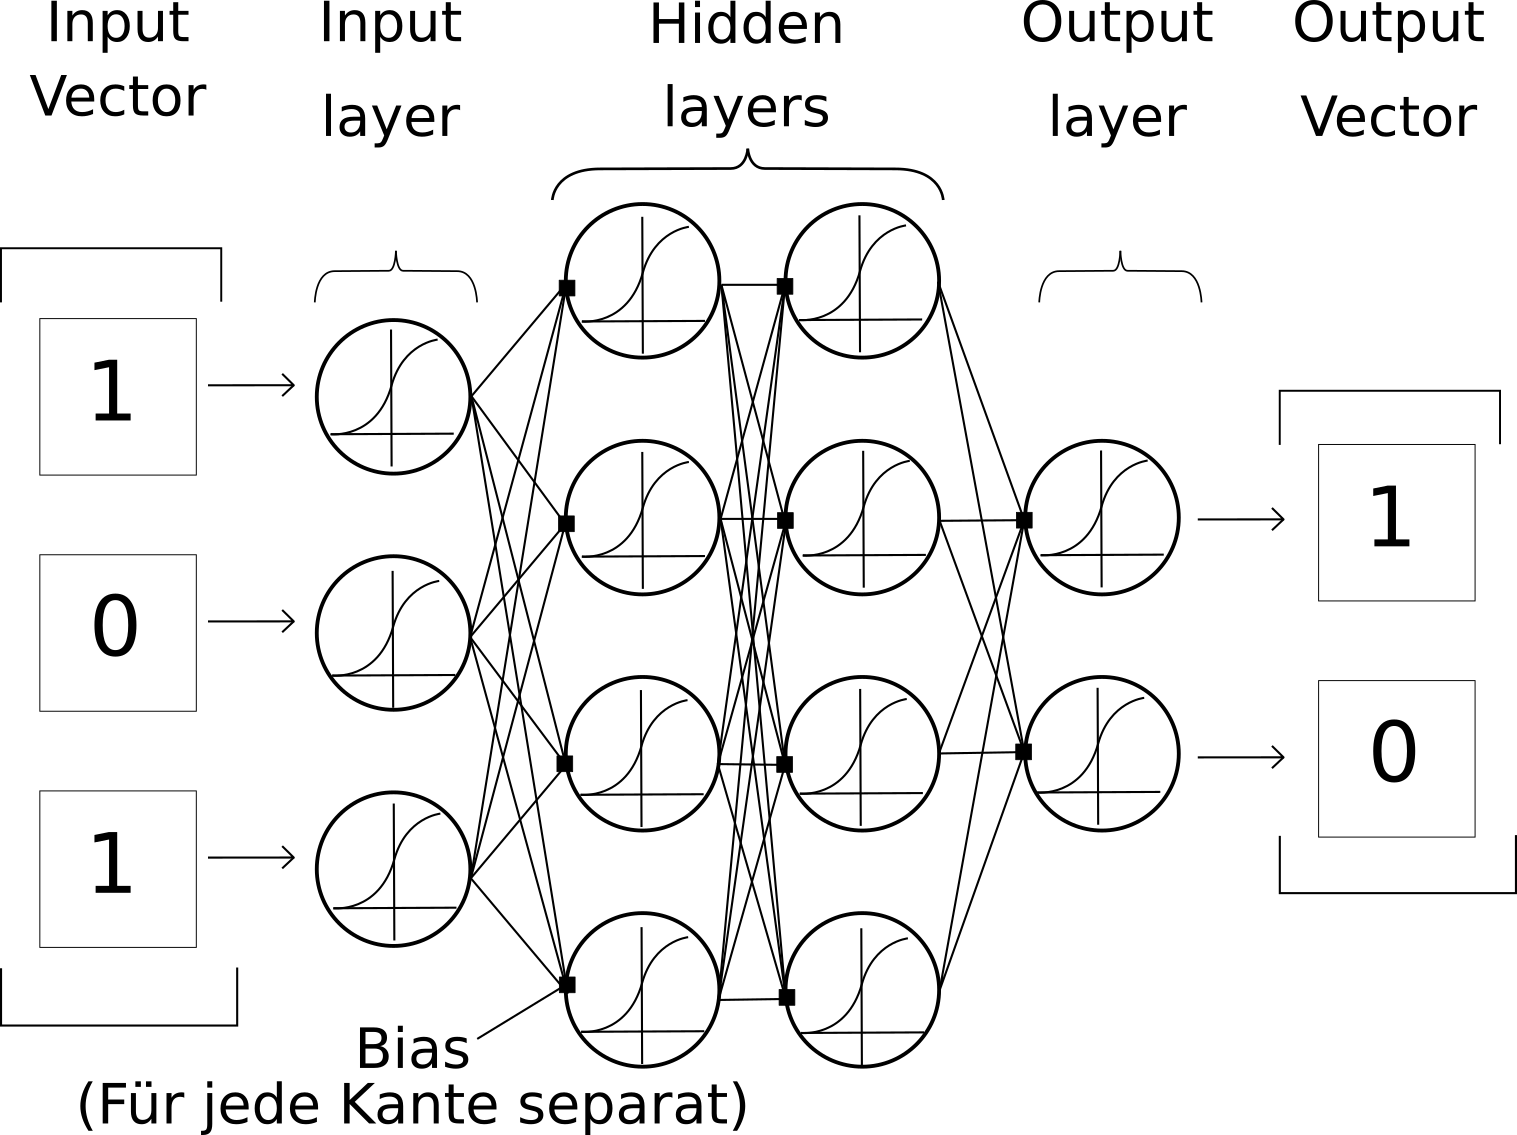
\includegraphics[width=\linewidth]{../graphics/Neural_Net.png}
\caption{Ein einfaches neuronales Netz}
\end{figure}
Jedes Neuron hat außerdem eine sogenannte Aktivierungsfunktion, die sich von Neuron zu Neuron unterscheiden kann, und jede Kante eine asoziierte Gewichtung und einen Bias. Ein neuronales Netz besteht also aus:\newline
\begin{enumerate}
	\item Neuronen mit gegebenenfalls verschiedenen Aktivierungsfunktionen, aufgeteilt in ein Input-, beliebig viele Hidden- und ein Output-Layer.
	\item Verbindungen zwischen diesen Neuronen, die jeweils einen eigenen Bias und eine Gewichtung besitzen.
\end{enumerate}
Sind alle Neuronen eines Layers jeweils mit allen Neuronen des nächsten Layers verbunden, wird das Layer als \glqq fully connected layer'' bezeichnet.
\subsection{Berechnung des Ausgabevektors}
Der Ausgabevektor wird berechnet, indem:
\begin{enumerate}
	\item Alle Ausgaben aus der vorherigen Schicht mit der Gewichtung der korrespondierenden Kante multipliziert werden
	\item Alle gewichteten Eingabewerte summiert werden
	\item Der Bias des Neurons hinzuaddiert wird
	\item Die Aktivierungsfunktion auf diesen Wert angewandt wird
\end{enumerate}
Die Aktivierungsfunktion hat dabei die Rolle die Werte zu normieren. Sie sorgt also dafür, dass alle Werte innerhalb des Netzes im Intervall $[0, 1]$ bleiben. Es gibt eine Vielzahl von Aktivierungsfunktionen. Die häufigste ist die sogenannte \glqq Sigmoid'' Funktion:
\begin{figure}[h]
\begin{center}
\begin{tikzpicture}
	\begin{axis}[samples=100, width=0.5\linewidth]
		\addplot[blue]{tanh(x)};
	\end{axis}
\end{tikzpicture}
\end{center}
\caption{Der Plot der Sigmoid Funktion $\sigma(x)=\frac{e^x}{e^x+1}$}
\end{figure}
\newline
Im Gegensatz dazu haben Gewichtungen typischerweise etwa den doppelten Wert der Eingaben. Alle Were werden jedoch automatisch im Lernprozess angepasst.
\newline
Der Begriff Eingabe- und Ausgabevektor lassen bereits vermuten, dass es sich bei Neuronalen Netzen um Objekte aus dem Bereich der linearen Algebra handelt. Daher wird im Folgenden auch die Notationsweise mit Hilfe von linearer Algebra verwendet. Betrachtet man eine Ausgabe eines Neurons wird diese als $a^ {(layer)}_{neuron}$ bezeichnet. Den Ausgabevektor des Input Layers würde man also folgendermaßen schreiben:
\begin{equation*}
\begin{bmatrix}
	a^0_0\\
	a^0_1\\
	a^0_2\\
	\vdots\\
	a^0_n
\end{bmatrix}
\end{equation*}
Die Gewichtungen $w$ der jeweiligen Kanten werden notiert als $w^{(von\ Layer)}_{(zu\ Neuron, von\ Neuron)}$. \glqq von Layer'' bezeichnet dabei das Layer in dem das Neuron liegt, das die Information ausgibt. \glqq zu Neuron'' ist der Index des Neurons im nächsten Layer, das die Information annimmt und \glqq von Neuron'' der Index des Neurons, das die Information abgibt. Die Gewichtung der Kante, die das zweite Neuron im ersten Layer mit dem dritten Neuron im zweiten Layer verebindet würde also als $w^0_{3,2}$ bezeichnet werden. Dabei wird bei null begonnen zu zählen, sodass das erste Layer und das erste Neuron den Index 0 erhält.\newline
Die Gewichtungen aller Verbindungen eines Layers zum nächsten können also als folgende Matrix geschrieben werden:
\begin{equation*}
	\begin{bmatrix}
	w_{0,0} & w_{0,1} & \cdots & w_{0,n}\\
	w_{1,0} & w_{1,1} & \cdots & w_{1,n}\\
	\vdots & \vdots & \ddots & \vdots\\
	w_{k,0} & w_{k,1} & \cdots & w_{k,n}\\
	\end{bmatrix}
\end{equation*}
Dabei ist $n$ hier die selbe Zahl wie $n$ im Ausgabevektor, da genau so viele Ausgaben vorhanden sein müssen, wie Neuronen in diesem Layer vorhanden sind, da jedes Neuron einen Wert ausgibt.\footnote{Es existieren auch Neuronen, die Daten verwerfen. Diese kommen im hier betrachteten Typ von neuronalem Netz allerdings nicht vor und werden daher der Einfachheit halber außenvor gelassen.}Der Bias Vektor wird genau so wie der Ausgabevektor bezeichnet.
\begin{equation*}
\begin{bmatrix}
	b^0_0\\
	b^0_1\\
	b^0_2\\
	\vdots\\
	b^0_n
\end{bmatrix}
\end{equation*}
Beachtet man jetzt noch, dass bei jedem Neuron die Aktivierungsfunktion angewandt werden muss ergibt sich folgende Gleichung für die Berechnung des Ausgabevektors $\vec{o}$ aus einem Einbagevektor $\vec{a}$ durch eine Schicht von Neuronen:
\begin{figure}[h]
	\begin{equation*}
		\vec{o} = \sigma\left(
		\begin{bmatrix}
			w_{0,0} & w_{0,1} & \cdots & w_{0,n}\\
			w_{1,0} & w_{1,1} & \cdots & w_{1,n}\\
			\vdots & \vdots & \ddots & \vdots\\
			w_{k,0} & w_{k,1} & \cdots & w_{k,n}\\
		\end{bmatrix}
		\begin{bmatrix}
			a^0_0\\
			a^0_1\\
			a^0_2\\
			\vdots\\
			a^0_n
		\end{bmatrix}
		+
		\begin{bmatrix}
			b^0_0\\
			b^0_1\\
			b^0_2\\
			\vdots\\
			b^0_n
		\end{bmatrix}
		\right)
	\end{equation*}
	\caption{Formel zur Berechnung eines Ausgabevektors aus einem Eingabevektor durch ein Layer Neuronen. }
\end{figure}
\newline
Zur Vereinfachung wurde die Funktion hier auf den gesamten Ausgabevektor angewandt. Dies ist korrekt, sofern alle Neuronen eines Layers die selbe Aktivierungsfunktion aufweisen. Dies muss natürlich nicht immer so sein. Sind die Aktivierungsfunktionen der Neuronen eines Layers verschieden, so wird die Aktivierungsfunktion des jeweiligen Neurones separat auf das korrespondierende Element des Vektors $W\cdot\vec{a}+\vec{b}$ angewandt.
\subsection{Der Lernprozess}
Der Lernprozess gliedert sich in wenige wesentliche Schritte. Zuerst wird unter Verwendung des oben beschriebenen Prozesses aus einem Eingabevektor ein Ausgabevektor berechnet. Diese Berechnung wird im Lernprozess extrem oft durchgeführt, weshalb sich neuronale Netze besonders schnell auf Grafikkarten trainieren lassen. Diese sind für mathematische Operationen im Bereich der linearen Algebra, wie Matritzenmultiplikation oder Addition optimiert und werden daher auch als Vektorprozessoren bezeichnet.\newline
Dieser Ausgabevektor wird nun, mit Hilfe einer Fehlerfunktion, mit dem erwarteten Ausgabevektor verglichen. Je größer dabei die Differenz zwischen erwartetem Ausgabevektor und tatsächlichem Ausgabevektor ist, desto größer ist der Wert der Fehlerfunktion. Der Ausgabewert dieser Fehlerfunktion wird als \glqq Fehler'' oder auch als \glqq Kosten'' bezeichnet. Wenn also das Minimum dieser Fehlerfunktion bestimmt wird, wird der Fehler minimiert und die tatsächliche Ausgabe des Netzes nähert sich der korrekten Ausgabe immer weiter an.\newline
Eine Methode, die hier erläutert werden soll, dieses Minimum zu finden ist das Gradientenverfahren. Nachdem mit Hilfe dieses Verfahrens der Fehler mimnimiert wurde, werden die Parameter, also die Gewichtungen und Biases, des neuronalen Netzes entsprechend angepasst. Diesen Prozess der Fehlerminimierung mittels des Gradientenverfahrens und der anschließenden Anpassung der Werte bezeichnet man auch als \glqq Backpropagation''. Es existieren auch noch andere Verfahren zur Fehlerminimierung, der Einfachheit halber soll hier aber nur Backpropagation erläutert werden.
\subsection{Fehlerfunktionen}
Es existiert eine Vielzahl von Fehlerfunktionen, die alle für unterschiedliche Anwendungsgebiete unterschiedlich passend sind. Im Groben lassen sich allerdings Fehlerfunktionen, die für Klassifizierungsprobleme geeignet sind von solchen unterscheiden, die für Regressionsprobleme geeignet sind.
\subsubsection{MSE -- Durchschnittlicher quadratischer Fehler}
Der sogenannte durchschnittliche quadratische Fehler ist eine häufig genutzte Fehlerfunktion für Regressionsprobleme. Die englische Bezeichnung lautet \glqq Mean squared error'', woraus sich auch die Abkürzung \glqq MSE loss'' ergibt. Sie ist wie in Abbildung \ref{MSE_equation} dargestellt, definiert.
\begin{figure}[h]
	\begin{equation*}
		MSE=\dfrac{\sum\limits_{i=1}^n(y_i-\hat{y_i})^2}{n}
	\end{equation*}
	\caption{Die Gleichung für den durchschnittlichen quadratischen Fehler}
	\label{MSE_equation}
\end{figure}
\newline
Wie der Name vermuten lässt, gibt diese Fehlerfunktion den Durchschnitt der quadrierten Differenzen zwischen dem vorausgesagten und dem tatsächlichen Ergebnis an. Aufgrund der Quadrierung des Fehlers, werden durch diese Funktion stark abweichende Werte wesentlich stärker gewichtet, als weniger stark abweichende Werte. Ihr Gradient ist außerdem einfach berechenbar, was für das Gradientenverfahren später relevant ist.\cite{3}
\subsubsection{MAE -- Durchschnitztlicher absoluter Fehler}
Bei dem durchschnittlichen absoluten Fehler handelt es sich ebenfalls um eine Fehlerfunktion, die für Regressionsprobleme eingesetzt wird. Die englische Bezeichnung lautet \glqq Mean absolute error''. Sie ist ähnlich wie der durchschnittliche quadratische Fehler definiert.
\begin{figure}[h]
	\begin{equation*}
	MAE=\dfrac{\sum\limits_{i=1}^n|y_i-\hat{y_i}|}{n}
	\end{equation*}
	\caption{Die Gleichung für den durchschnittlichen absoluten Fehler}
	\label{MAE_equation}
\end{figure}
\newline
Auch hier wird die \glqq Richtung'' des Fehlers, in diesem Fall durch die Normierung, verworfen. Außerdem ist diese Fehlerfunktion nicht so anfällig gegenüber Ausreißern in den Daten, da dieser Fehler nicht quadriert wird. Ein Nachteil des durchschnittlichen absoluten Fehlers ist allerdings die höhere Komplexität zur Berechnung des Gradienten.\cite{3}
\subsubsection{Kreuzentropiefehler}
Der Kreuzentropiefehler ist die am häufigsten verwendete Fehlerfunktion für Klassifizierungsprobleme. Sie gibt den Fehler für eine Klassifizierung an, die den gegebenen Klassen Wahrscheinlichkeiten im Intervall $I=[0;1]$ zuordnet. Dabei steigt der Fehler stärker, je weiter sich die Vorhersage vom tatsächlichen Wert entfernt. Wie aus Abbildung \ref{CEL_Graph} hervorgeht, wird also sicheren, aber falschen Vorhersagen der höhste Fehlerwert zugeordnet. 
\begin{figure}[h]
	\begin{center}
		\begin{tikzpicture}
		\begin{axis}[width=0.7\linewidth, 
		xmax=1, 
		ymax=10, 
		xmin=0, 
		samples=10,
		xlabel={vorhergesagte Wahrscheinlichkeit},
		ylabel={Kreuzentropiefehler}]
		\addplot[blue]{-ln(x))};
		\end{axis}
		\end{tikzpicture}
	\end{center}
	\caption{Der Graph der Kreuzentropie Fehlerfunktion wenn das tatsächliche Label 1 ist}
	\label{CEL_Graph}
\end{figure}
\newline
Der Fehler steigt also mit zunehmender Abweichung der Vorhersage zum tatsächlichen Label rapide an.\newline 
Mathematisch ist der Kreuzentropiefehler nach der Funktion in Abbildung \ref{CEL_Function} definiert, wobei $y$ einen Binärindikator darstellt, der angibt ob das zu klassifizierende Objekt tatsächlich zur Klasse gehört (dann ist er 1) und $p$ die vorausgesagte Wahrscheinlichkeit ob das Objekt zur Klasse gehört, beschreibt.
\begin{figure}[h]
	\begin{equation*}
	CrossEntropyLoss=-(yln(p)+(1-y)ln(1-p))
	\end{equation*}
	\caption{Die Gleichung für den Kreuzentropiefehler}
	\label{CEL_Function}
\end{figure}
\newline
Hier fällt auf, dass, falls das Label 0 ist, der linke Teil der Gleichung weg fällt und falls es 1 ist, der Rechte. Wenn berechnetes und tatsächliches Label identisch sind, ist der Fehler stets 0.\newline
Existieren mehr als 2 Klassen, handelt es sich also nicht mehr um eine Binärklassifizierung, müssen die Fehler nach der Gleichung in Abbildung \ref{CEL_Finction_cummulative} summiert werden.
\begin{figure}[h]
	\begin{equation*}
	CrossEntropyLoss(M)=-\sum\limits_{c=1}^My_{o,c}ln(p_{o,c})
	\end{equation*}
	\caption{Die Gleichung für den durchschnittlichen absoluten Fehler}
	\label{CEL_Finction_cummulative}
\end{figure}
\newline
Dabei gibt M die Anzahl der Klassen an, c das Label für die Klasse und o die berechnete Klassifizierung für diese Klasse.
\subsection{Gradientenverfahren und Backpropagation}
Das Gradientenverfahren ist ein Verfahren um das Minimum einer Funktion zu finden. Die Funktion, deren Minimum gefunden werden soll ist in diesem Fall die Fehlerfunktion. Diese ist von allen Gewichtungen und Biases des Netzwerkes abhängig, da sie direkt vom Ausgabevektor des Netzes abhängig ist. Der Gradient dieser Funktion ist in Abbildung \ref{Gradient_Function} dargestellt.
\begin{figure}[h]
	\begin{equation*}
	\nabla C(w_1,b_1,\ldots,w_n,b_n)=
	\begin{bmatrix}
		\frac{\partial C}{\partial w_1}\\
		\frac{\partial C}{\partial b_1}\\
		\vdots\\
		\frac{\partial C}{\partial w_n}\\
		\frac{\partial C}{\partial b_n}
	\end{bmatrix}
	\end{equation*}
	\caption{Die Gleichung für den Gradienten der Fehlerfunktion}
	\label{Gradient_Function}
\end{figure}
\newline
Um also das Ergebnis \glqq richtiger'' zu machen, müssen alle Gewichtungen und Biases negativ zu diesem Gradienten angepasst werden, da der Gradient ja den Hochpunkt angibt. Diese Anpassung erfolgt, indem das Netz vom Ausgabelayer an, deshalb heißt das Verfahren Backpropagation, durchgegangen wird, und die Gewichtungen und Biases angepasst werden.\newline
Oft wird zur Verbildlichung des Gradientenverfahrens die Analogie eines Balles verwendet, der einen Hügel hinunter rollt. Er findet den Tiefpunkt indem er hinab rollt und dabei immer automatisch eine Kraft nach unten wirkt.
\subsubsection{Lernrate}
Eine wichtige Rolle dabei spielt die sogenannte \glqq Lernrate'' $\eta$, mit der die Änderung nach der Formel in Abbildung \ref{Learning_Rate_Function} berechnet wird.
\begin{figure}[h]
	\begin{equation*}
	w^n_{neu}=w^n_{alt}-\eta\times\frac{\partial C}{\partial w^n}
	\end{equation*}
	\caption{Die Gleichung für die Anpassung eines einzelnen Parameters}
	\label{Learning_Rate_Function}
\end{figure}
\newline
Diese Lernrate ist notwendig um nicht über das Minimum \glqq hinweg zu springen''. Sollte sie zu groß sein, passiert genau dies, da die Anpassungen der Parameter in zu großen Schritten erfolgt. Sollte sie hingegen zu klein sein, lernt das Netz sehr langsam. Typische Werte sind abhängig von der zu erlernenden Aufgabe, liegen jedoch in der Regel bei etwa 0.01 bis 0.0001 \footnote{Dies ist ein bloßer Erfahrungswert. Maschinelles Lernen erfordert oft sehr viele Versuche, weshalb nicht genau festgelegt werden kann, wann welche Lernrate optimal ist.}.
\begin{figure}[h]
	\begin{center}
		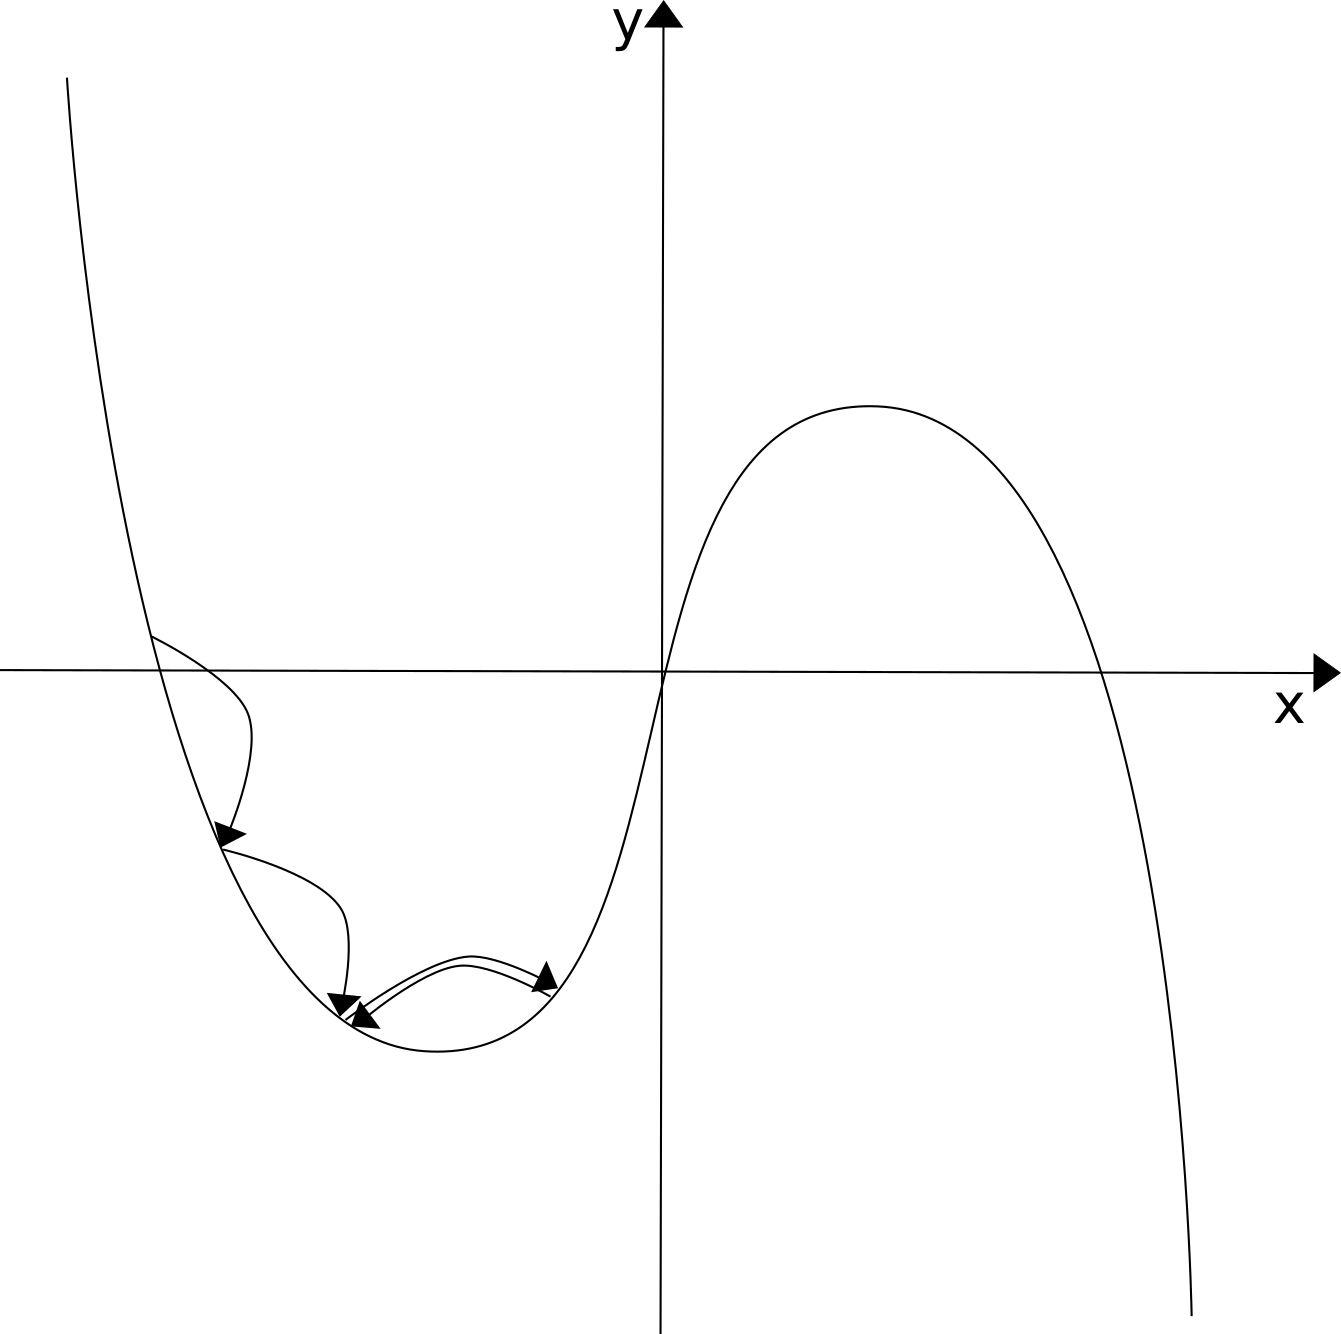
\includegraphics[width=0.5\linewidth]{../graphics/gdf_big_lr.png}
	\end{center}
	\caption{$\eta$ ist hier zu groß gewählt}
	\label{Learning_Rate_Graphic}
\end{figure}
\newline
Abbildung \ref{Learning_Rate_Graphic} stellt dar, wieso das Minimum nicht erreicht werden kann, falls die Lernrate zu groß gewählt wurde. Es ist zu sehen, dass der Parameter immer gleich viel geändert wird und dabei das Minimum übersprungen wird, da die Lernrate konstant zu groß ist. Dieses Problem kann behoben werden indem eine adaptive Lernrate verwendet wird. Dabei verringert sich die Lernrate im Laufe des Lernprozesses, sodass zu Beginn die Vorzüge des schnellen Lernens genutzt werden können und am Ende trotzdem ein hoher Grad an Präzision erreicht werden kann.
\subsection{Verschiedene Layerarten}
Mit Hilfe von maschinellem Lernen lassen sich eine Vielzahl von Aufgaben bewältigen. Entsprechend komplex müssen Neuronale Netze aber auch sein. Demzufolge ist es notwendig, Neuronen zu entwickeln, die andere Fähigkeiten aufweisenl, als das einfache oben im sogenannten \glqq Linear Layer'' verwendete Neuron. Da man in der Regel nur eine Art von Neuron in einem Layer verwendet, wird das gesamte Layer nach der verwendeten Neuronenart benannt. Die unten beschriebenen Layerarten werden vor allem in einer Klasse von neuronalen Netzen verwendet, die als \glqq Convolutional neural networks'' bezeichnet werden. Sie werden meißt im Bereich der komplexen fragmentbasierten Bilderkennung eingesetzt, da sie besonders gut geeignet sind um Kanten oder gewisse Teile eines Bildes, wie zum Beispiel Merkmale eines Gesichtes, zu erkennen.
\subsubsection{Convolutional Layers}
Convolutional Layers weisen eine fundamental andere Funktionsweise als lineare Layers auf. Sie nehmen zwar ebenfalls rationale Zahlen an und geben rationale Zahlen aus \footnote{Im Folgenden werden 2 Dimensionale convolutional Layers betrachtet, da diese einfacher vorstellbar sind. Sie nehmen dann eine Matrix rationaler Zahlen an und geben auch eine Matrix rationaler Zahlen aus. Dies korrespondiert mit dem Anwendungsbereich der Erkennung von schwarz weiß Bildern.}, berechnen die Ausgabe jedoch nicht nur mit Hilfe einer Aktivierungsfunktion sondern unter der Verwendung sogenannter \glqq Filter''. Diese Filter sind eine $m\times n$ große Matrix, die auch als \glqq Kernel'' bezeichnet wird. Der Kernel wird dabei über die Eingabematrix bewegt (daher der Name convolution) und erzeugt eine Ausgabematrix. Dafür wird der betrachtete Abschnitt der Eingabematrix $A$ und des Kernels $B$ skalar multipliziert wobei das Skalarprodukt als Frobenius-Skalarprodukt, also als
\begin{equation*}
	\langle A, B\rangle=\sum_{i=1}^{m}\sum_{j=1}^{n}a_{ij}b_{ij}
\end{equation*} 
definiert ist. Die Matritzen werden also Komponentenweise multipliziert und diese Produkte dann summiert.\newline
Dies ist in Abbildung \ref{Convolution_illustration} verbildlicht.
\begin{figure}[h]
	\begin{center}
	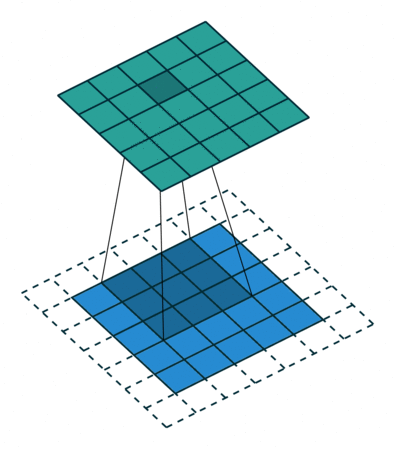
\includegraphics[width=0.2\linewidth]{../graphics/conv/conv008.png}
	\end{center}
	\caption[Eine Verbildlichung der Vorgänge in einem convolutional Layer\newline
	Aus einer Animation von\newline
	https://github.com/vdumoulin/conv\_arithmetic/blob/master/README.md\\
	Vincent Dumoulin, Francesco Visin - A guide to convolution arithmetic for deep learning (BibTeX)]{Eine Verbildlichung der Vorgänge in einem convolutional Layer. Das blaue Raster stellt die Eingabe dar, das grüne die Ausgabe.}
	\label{Convolution_illustration}
\end{figure}
\newpage
Ein Filter kann ganz verschiedene Werte aufweisen. So können Filter der Form 
\begin{figure}[h]
	\begin{minipage}{0.2\linewidth}
		\centering
		\begin{equation*}
			\begin{bmatrix}
			-1 & -1 & -1\\
			1 & 1 & 1\\
			0 & 0 & 0
			\end{bmatrix}
		\end{equation*}
		\caption{Erkennt obere horizontale Kanten}
	\end{minipage}
	\hfill
	\begin{minipage}{0.2\linewidth}
		\centering
		\begin{equation*}
			\begin{bmatrix}
			-1 & 1 & 0\\
			-1 & 1 & 0\\
			-1 & 1 & 0
			\end{bmatrix}
		\end{equation*}
		\caption{Erkennt linke vertikale Kanten}
	\end{minipage}
	\hfill
	\begin{minipage}{0.2\linewidth}
		\centering
		\begin{equation*}
			\begin{bmatrix}
			0 & 0 & 0\\
			1 & 1 & 1\\
			-1 & -1 & -1
			\end{bmatrix}
		\end{equation*}
		\caption{Erkennt untere horizontale Kanten}
	\end{minipage}
	\hfill
	\begin{minipage}{0.2\linewidth}
		\centering
		\begin{equation*}
			\begin{bmatrix}
			0 & 1 & -1\\
			0 & 1 & -1\\
			0 & 1 & -1
			\end{bmatrix}
		\end{equation*}
		\caption{Erkennt rechte vertikale Kanten}
	\end{minipage}
\end{figure}
\newline
beispielsweise zur einfachen Kantenerkennung genutzt werden. Zur Veranschaulichung wurden diese Filter auf das Beispielbild in Abbildung \ref{Filter_Example_raw} angewandt. Das Ergebnis ist in Abbildung \ref{Filter_output dargestellt} dargestellt.
\begin{figure}[h]
	\begin{center}
		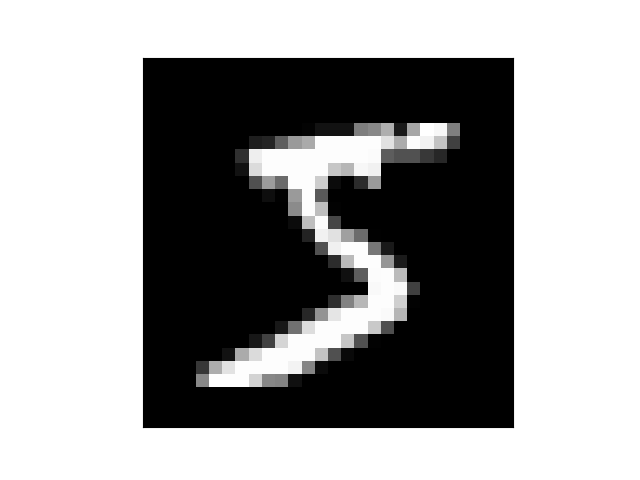
\includegraphics[width=0.5\linewidth]{../graphics/mnist_5/mnist_5_raw.png}
		\caption{Das Beispielbild aus dem Mnist Datensatz}
		\label{Filter_Example_raw}
	\end{center}
\end{figure}
\\
\begin{figure}[h]
	\begin{minipage}{0.2\linewidth}
		\centering
		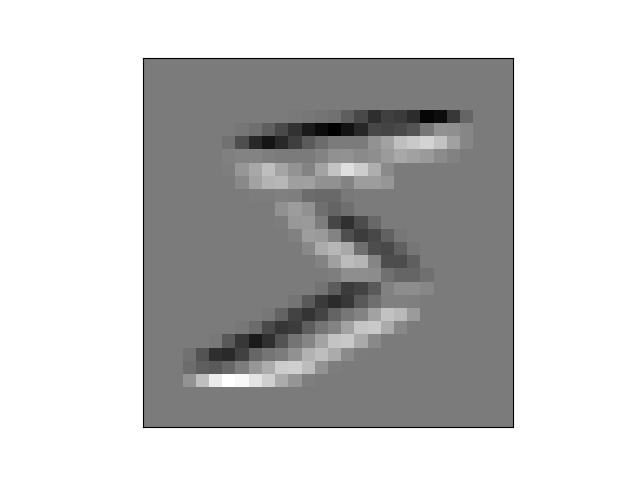
\includegraphics[width=\linewidth]{../graphics/mnist_5/mnist_5_upper_edges.png}
	\end{minipage}
	\hfill
	\begin{minipage}{0.2\linewidth}
		\centering
		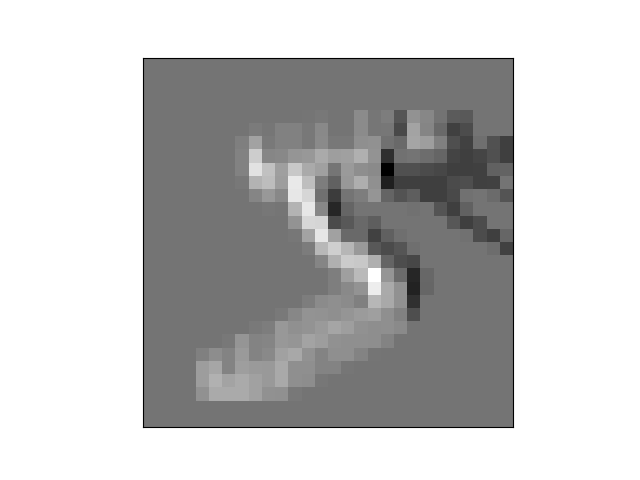
\includegraphics[width=\linewidth]{../graphics/mnist_5/mnist_5_left_edges.png}
	\end{minipage}
	\hfill
	\begin{minipage}{0.2\linewidth}
		\centering
		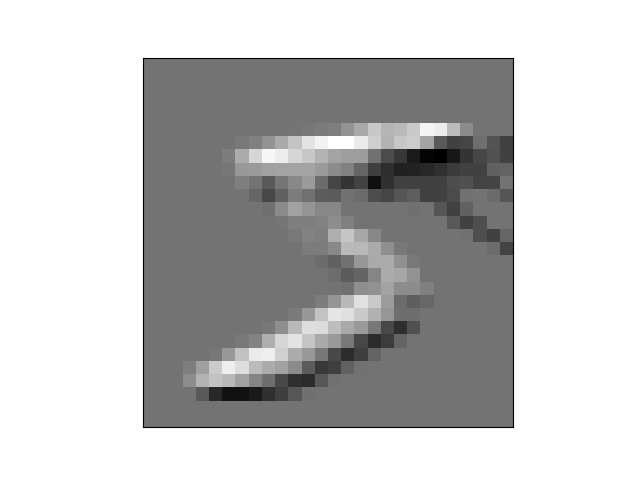
\includegraphics[width=\linewidth]{../graphics/mnist_5/mnist_5_lower_edges.png}
	\end{minipage}
	\hfill
	\begin{minipage}{0.2\linewidth}
		\centering
		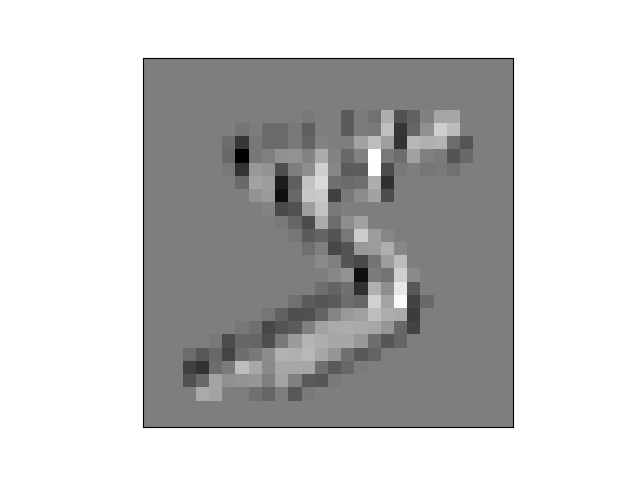
\includegraphics[width=\linewidth]{../graphics/mnist_5/mnist_5_right_edges.png}
	\end{minipage}
\caption{Die jeweils oben stehenden Filter wurden auf das Beispielbild angewandt.}
\label{Filter_output dargestellt}
\end{figure}
\\
Der jeweils dunkel dargestellte Bereich kann als das identifiziert werden, was vom convolutional Layer als Kante erkannt wurde. Hier werden eindeutige Limitationen deutlich: Es kann nur als Kante erkannt werden, was auch eindeutig senkrecht oder waagerecht ist. Außerdem kann es zu Fehlentscheidungen kommen.\\
Die Kernels werden natürlich nicht per Hand initialisiert und angepasst, sondern setzen sich aus Parameternm zusammen, die im Laufe des Lernprozesses durch das Netz anpassbar sind. Das Netz kann also die Filtermatrix selber verändern. Die Filter werden meißt mit Zufallswerten initialisiert und dann während des Lernens  angepasst. Ferner muss ein Kernel auch nicht immer drei Einheiten breit sein, sondern kann jede Größe $\ge2$ annehmen. Je nachdem, wie sich der Kernel über die Eingabematrix bewegt, ist außerdem ein sogenanntes \glqq Padding'' nötig, da gegebenenfalls Werte betrachtet werden müssten, die nicht in der Eingabematrix liegen. In der Regel werden daher alle Werte, die nicht in der Eingabematrix vorhanden sind durch 0 ersetzt. Das Padding ist in Abbildung \ref{Convolution_illustration} als weiß in der Eingabematrix dargestellt. Es ist eine Art \glqq Rand aus Nullen'', der um dasd Bild gelegt wird.\\ 
\\
Hintereinander können convolutional Layers auch ganze Elemente eines Bildes erkennen. Erkennt das erste Layer wie oben gezeigt beispielsweise Kanten, so kann das Layer darauf Kombinationen aus diesen, wie beispielsweise Ecken oder Winkel, erkennen. Wie gefilterte Bilder für sogenannte \glqq High-Level-Features'' aussehen können ist in Abbilldung \ref{HL_features_conv} dargestellt. 
\begin{figure}[h]
	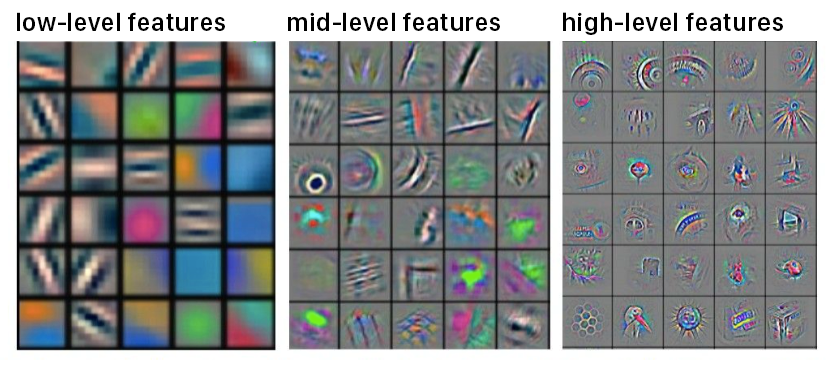
\includegraphics[width=\linewidth]{../graphics/features.png}
	\caption[Beispiele für low- mid- und high-level Features in Convolutional Neural Nets\newline
	Quelle: https://tvirdi.github.io/2017-10-29/cnn/]{Beispiele für low- mid- und high-level Features in Convolutional Neural Nets}
	\label{HL_features_conv}
\end{figure}
Das bemerkenswerte an Convolutional Layers ist vor allem, dass duch ähnliche Optimierungsalgorytmen auch hier maschinelles lernen möglich ist, dass sich ein neuronales Netz diese Filter also selbstständig beibringen kann.
\subsubsection{Pooling Layers}
\section{PyTorch}
\subsection{Datenvorbereitung}
\subsection{Definieren des Netzes}
\subsection{Trainieren des Netzes}
\section{Fallbeispiel I:\newline Ein Klassifizierungsnetzwerk für handgeschriebene Ziffern}
\subsection{Aufgabe}
\subsection{Der MNIST Datensatz}
\subsection{Fragmentbasierte Erkennung}
\subsection{Ergebnis}
\section{Fallbeispiel II:\newline Eine selbsttrainierende KI für Tic-Tac-Toe}
\subsection{Das Prinzip}
\subsection{Chance-Tree Optimierung}
\subsection{Lösung mittels eines neuronalen Netzes}
\subsection{Vergleich}
\section{Schlusswort}
\newpage
\begin{thebibliography}{99}
	\bibitem{1}
	Hands-On Machine Learning with Scikit-Learn and TensorFlow\newline
	von Aurélien Géron\newline
	Veröffentlicht: March 2017 O'Reilly Media, Inc\newline
	ISBN: 9781491962282
	\bibitem{2}
	Die Logistik des Lernens eine Studie der LMU München\newline
	Quelle: www.uni-muenchen.de/forschung/news/2013/\newline f-71-13\_kiebler\_nervenzellen.html --abgerufen am 16.11.2019
	\bibitem{3}
	Common Loss functions in machine learning\newline
	Von Ravindra Parmar\newline
	Veröffentlicht am 02.09.2018, abgerufen am 07.01.2020\newline
	Quelle: https://towardsdatascience.com/common-loss-functions-in-machine-learning-46af0ffc4d23 
	
\end{thebibliography}
\listoffigures
\end{document}